\HeadingLevelB{SGX Enclave Launch Control}
\label{sec:sgx_launch_control}

The SGX implementation contained in a CPU's hardware does not directly enforce
the enclave attribute checks that decide which enclaves can access the CPU
secrets used for software attestation. The potentially complex restrictions on
enclave attributes are instead enforced by the Launch Enclave, which is an
enclave issued by Intel that gets to approve every other enclave before it is
initialized by \textit{EINIT}~(\S~\ref{sec:sgx_einit_overview}). The officially
documented information about the approval process is discussed in
\S~\ref{sec:sgx_launch_enclave}.

% Enclave License
%   US 8,972,746 B2 - 34:6-23
% Licenses are evaluated into Permits (which became EINITTTOKEN)
%   US 8,972,746 B2 - 34:24-29, 35:27-59
% EINIT requires a Permit to launch a production enclave
%   US 8,972,746 B2 - 35:60-67, 36:1-3, 36:47-52, 38:4-65
% License Enclave creates Permit
%   US 8,972,746 B2 - 36:40-46, 37:50-67, 38:1-3
% EMKPERMIT seems to have gotten merged into EINIT
%   US 8,972,746 B2 - 36:53-67, 37:1-7, 37:24-49
% License became SIGSTRUCT
%   US 8,972,746 B2 - 37:8-23

The SGX patents~\cite{intel2013patent1, intel2013patent2} disclose in no
uncertain terms that the Launch Enclave was introduced to ensure that each
enclave's author has a business relationship with Intel, and implements a
software licensing system. \S~\ref{sec:sgx_licensing} briefly discusses the
implications, should this turn out to be true.


\HeadingLevelC{Enclave Attributes Access Control}
\label{sec:sgx_launch_enclave}

% ATTRIBUTES: SDM S 38.7.1

The security of SGX's software attestation scheme depends on denying
unauthorized enclaves access to the provisioning
keys~(\S~\ref{sec:sgx_quoting_enclave}) that can be used to obtain an
Attestation Key. This requirement translates into only allowing the
PROVISIONKEY attribute to be set for the enclaves that are trusted to carry out
the attestation process.

The logic embedded in the circuitry of SGX-enabled processors does not directly
control the use of the PROVISIONKEY attribute. Instead, the SGX design requires
that all enclaves be vetted by a \textit{Launch Enclave}~(LE) that implements
the access control checks needed for the PROVISIONKEY attribute, and for any
other privileged attributes that may be introduced in future designs.

The LE is only briefly mentioned in Intel's official documentation. Neither its
behavior nor its interface with the system software is specified. We speculate
that Intel has not been forthcoming about the LE because of its role in
enforcing software licensing, which will be discussed in
\S~\ref{sec:sgx_licensing}. This section ignores the licensing aspect, and
describes a minimal LE implementation, illustrated in
Figure~\ref{fig:sgx_einittoken}, which would satisfy SGX's security
requirements.

\begin{figure}[hbt!]
  \centering
  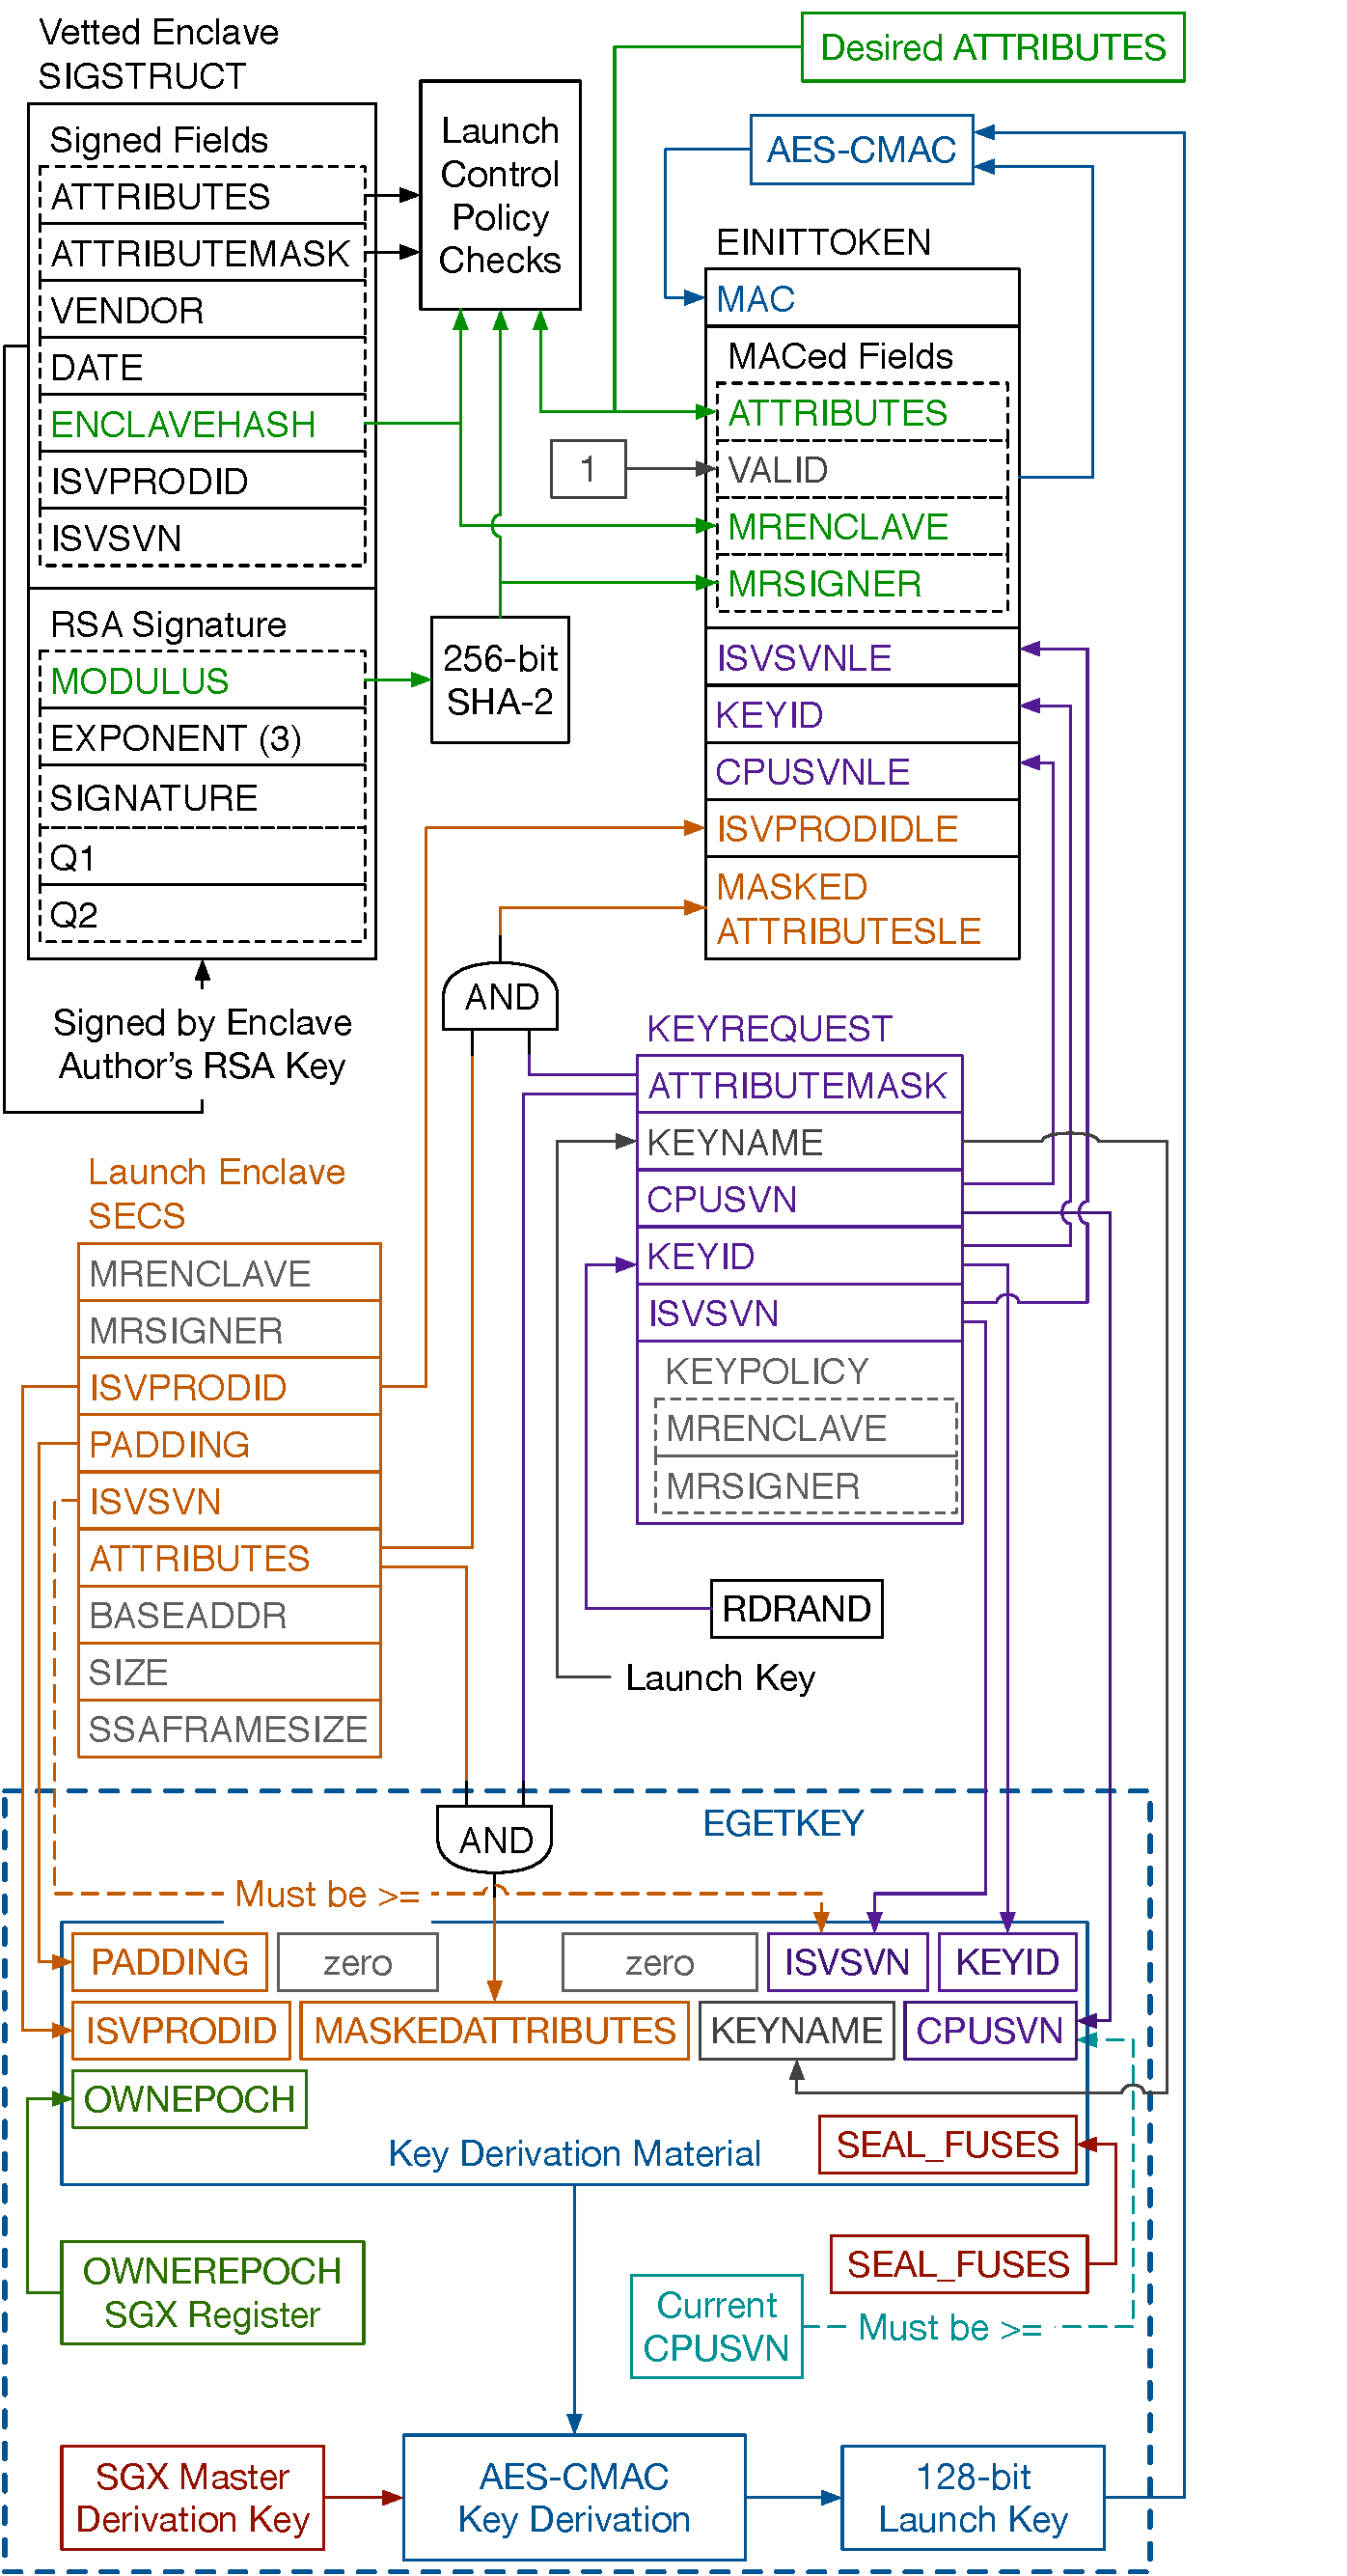
\includegraphics[width=95mm]{figures/sgx_einittoken.pdf}
  \caption{
    The SGX Launch Enclave computes the EINITTOKEN.
  }
  \label{fig:sgx_einittoken}
\end{figure}

% EINIT Token Structure (EINITTOKEN): SDM S 38.14

The LE approves an enclave by issuing an \textit{EINIT Token}~(EINITTOKEN) that
contains the approved enclave's
measurement-based~(\S~\ref{sec:sgx_measurement})
and certificate-based~(\S~\ref{sec:sgx_certificate_identity}) identities, just
like a local attestation REPORT~(\S~\ref{sec:sgx_ereport}). This token is
inspected by \texttt{EINIT}~(\S~\ref{sec:sgx_einit_overview}), which refuses to
initialize enclaves with incorrect tokens.

While an EINIT token is handled by untrusted system software, its integrity is
protected by a MAC tag~(\S~\ref{sec:integrity_crypto}) that is computed using a
\textit{Launch Key} obtained from \texttt{EGETKEY}. The \texttt{EINIT}
implementation follows the same key derivation process as \texttt{EGETKEY} to
convince itself that the EINITTOKEN provided to it was indeed generated by an
LE that had access to the Launch Key.

The SDM does not document the MAC algorithm used to confer integrity guarantees
to the EINITTOKEN structure. However, the \texttt{EINIT} pseudocode verifies
the token's MAC tag using the same function that the \textit{EREPORT} pseudocode
uses to create the REPORT structure's MAC tag. It follows that the reasoning in
\S~\ref{sec:sgx_ereport} can be reused to conclude that EINITTOKEN structures
are MACed using AES-CMAC with 128-bit keys.

% EGETKEY: SDM S 41.4.1
% Key Derivation: SDM Table 41-43

The \texttt{EGETKEY} instruction only derives the Launch Key for enclaves that
have the LAUNCHKEY attribute set to true. The Launch Key is derived using the
same process as the Seal Key~(\S~\ref{sec:sgx_egetkey}). The derivation material
includes the current enclave's versioning information (ISVPRODID and ISVSVN)
but it does not include the main fields that convey an enclave's identity,
which are MRSIGNER and MRENCLAVE. The rest of the derivation material follows
the same rules as the material used for Seal Keys.

The EINITTTOKEN structure contains the identities of the approved enclave
(MRENCLAVE and MRSIGNER) and the approved enclave attributes (ATTRIBUTES). The
token also includes the information used for the Launch Key derivation,
which includes the LE's Product ID (ISVPRODIDLE), SVN (ISVSVNLE), and the
bitwise AND between the LE's ATTRIBUTES and the ATTRIBUTEMASK used in the
KEYREQUEST (MASKEDATTRIBUTESLE).

The EINITTOKEN information used to derive the Launch Key can also be used
by \texttt{EINIT} for damage control, e.g. to reject tokens issued by Launch
Enclaves with known security vulnerabilities. The reference pseudocode supplied
in the SDM states that \texttt{EINIT} checks the DEBUG bit in the
MASKEDATTRIBUTESLE field, and will not initialize a production enclave using
a token issued by a debugging LE. It is worth noting that MASKEDATTRIBUTESLE is
guaranteed to include the LE's DEBUG attribute, because \texttt{EGETKEY} forces
the DEBUG attribute's bit in the attributes mask to 1
(\S~\ref{sec:sgx_egetkey}).

The check described above makes it safe for Intel's privileged key to sign
Launch Enclaves with debugging features enabled. Without this check, using a
privileged Intel signing key on a single debug LE could invalidate SGX's
security guarantees on all the CPU chips that accept that signing key.
Concretely, if the issued SIGSTRUCT would be leaked, any attacker could build a
debugging LE, use the SGX debugging features to modify the code inside it, and
issue tokens that authorize malicious enclaves to access the Provisioning Key
used by the software attestation process.

A further advantage of the check described above is that Intel can supply SGX
enclave developers with a debugging LE that performs minimal or no security
checks before issuing an EINITTOKEN. The debugging LE can be used to launch any
enclave with the DEBUG attribute set. The DEBUG attribute is always included in
\texttt{EGETKEY}'s key derivation material, so debugging enclaves cannot access
the symmetric keys used to encrypt the secrets of production enclaves.

% EINIT: SDM S 41.3
% EINITTOKENKEY is bit 5, INTEL_ONLY_MASK is 0x20

The enclave attributes access control system described above relies on the LE
to reject initialization requests that set privileged attributes such as
PROVISIONKEY on unauthorized enclaves. However, the LE cannot vet itself, as
there will be no LE available when the LE itself needs to be initialized.
Therefore, the Launch Key access restrictions are implemented in hardware.

\texttt{EINIT} accepts an EINITTOKEN whose VALID bit is set to zero, if
the enclave's MRSIGNER~(\S~\ref{sec:sgx_mrsigner}) equals a hard-coded value
that corresponds to an Intel public key. For all other enclave authors, an
invalid EINIT token causes \texttt{EINIT} to reject the enclave and produce an
error code.

This exemption to the token verification policy provides a way to bootstrap the
enclave attributes access control system, namely using a zeroed out EINITTOKEN
to initialize the Launch Enclave. At the same time, the cryptographic
primitives behind the MRSIGNER check guarantee that only Intel-provided
enclaves will be able to bypass the attribute checks. This does not change
SGX's security properties because Intel is already a trusted party, as it is
responsible for generating the Provisioning Keys and Attestation Keys used by
software attestation~(\S~\ref{sec:sgx_quoting_enclave}).

Curiously, the \texttt{EINIT} pseudocode in the SDM states that the instruction
enforces an additional restriction, which is that all enclaves with the
LAUNCHKEY attribute must have its certificate issued by the same Intel public
key that is used to bypass the EINITTTOKEN checks. This restriction appears to
be redundant, as the same restriction could be enforced in the Launch Enclave.


\HeadingLevelC{Licensing}
\label{sec:sgx_licensing}

The SGX patents~\cite{intel2013patent1, intel2013patent2} disclose that
\texttt{EINIT} Tokens and the Launch Enclave~(\S~\ref{sec:sgx_launch_enclave})
were introduced to verify that the SIGSTRUCT certificates associated with
production enclaves are issued by enclave authors who have a business
relationship with Intel. In other words, the Launch Enclave is intended to be
\textbf{an enclave licensing mechanism that allows Intel to force itself as an
intermediary in the distribution of all enclave software}.

The SGX patents are likely to represent an early version of the SGX design, due
to the lengthy timelines associated with patent application approval.
In light of this consideration, we cannot make any claims about Intel's current
plans. However, given that we know for sure that Intel considered enclave
licensing at some point, we briefly discuss the implications of implementing
such a licensing plan.

First, implementing license checks in the Launch Enclave will increase the
complexity of the enclave's code. The production Launch Enclave is incredibly
security-sensitive, as a vulnerability in its code has the potential for
allowing attackers to give malicious enclaves access to the Provisioning Key
that is the base of SGX's software attestation
process~(\S~\ref{sec:sgx_quoting_enclave}). Increasing the complexity of such a
security-sensitive piece of code seems rather reckless.

This first concern can be somewhat mitigated by delegating the actual license
checks to another enclave, and using a MAC scheme to verify the authenticity of
the result received from that enclave.

Second, a much bigger concern about implementing enclave licensing is that
Intel has a near-monopoly on desktop and server-class processors, and being
able to decide which software vendors are allowed to use SGX can effectively
put Intel in a position to decide winners and losers in many software markets.

Assuming SGX reaches widespread adoption, this issue is the software security
equivalent to the Net Neutrality debates that have pitted the software industry
against telecommunication giants. Given that virtually all competent software
development companies have argued that losing Net Neutrality will stifle
innovation, it is fairly safe to assume that Intel's ability to regulate access
to SGX will also stifle innovation.

Furthermore, from a historical perspective, the enclave licensing scheme
described in the SGX patents is very similar to Verified Boot, which was
briefly discussed in \S~\ref{sec:sgx_related_tpm}. Verified Boot has mostly
received negative reactions from software developers, so it is likely that an
enclave licensing scheme would meet the same fate, should the developer
community become aware of it.


\HeadingLevelC{Policing Provisioning Keys}
\label{sec:sgx_provisioning_privacy}

The derivation material for Provisioning keys does not include OWNEREPOCH, so
malicious enclaves can potentially use these keys to track a CPU chip package
as it exchanges owners. For this reason, the SGX design includes a simple
access control mechanism that can be used by system software to limiting
enclave access to Provisioning keys. \texttt{EGETKEY} refuses to derive
Provisioning keys for enclaves whose PROVISIONKEY attribute is not set to true.

The SGX instructions used to load and initialize enclaves introduced in
\S~\ref{sec:sgx_enclave_lifecycle} (\texttt{ECREATE}, \texttt{EADD},
\texttt{EINIT}) can only be issued by privileged system software, because they
manage the EPC. This privilege requirement gives the system software an ability
to filter the enclaves that run on a computer.


\S~\ref{sec:sgx_einit_overview}

The system software that provides the enclave loading
service which issues the \texttt{EINIT}~(
instruction can protect the computer owner's privacy by
enclaves


\HeadingLevelC{Enclaves Cannot DOS the System Software}
% NOTE: This is a slightly edited answer to a question we received.

SGX enclaves execute at the lowest privilege level (user mode / ring 3), so
they cannot compromise the system software without exploiting a security
vulnerability. Therefore, the only kind of malicious behavior that an enclave
can exhibit is denial of service (DoS).

The SGX design provides system software the tools it needs to protect itself
from enclaves that engage in CPU hogging and DRAM hogging. As enclaves cannot
perform I/O directly, these are the only two classes of DoS attacks available
to them.

An enclave that attempts to hog an LP assigned to it can be preempted by the
system software via an Inter-Processor Interrupt~(IPI,~\S~\ref{sec:interrupts})
issued from another processor. This method is available as long as the system
software reserves at least one LP for non-enclave computation.

Furthermore, most OS kernels use tick schedulers, which use a real-time clock
(RTC) configured to issue periodical interrupts (ticks) to all cores. The RTC
interrupt handler invokes the kernel's scheduler, which chooses the thread that
will get to use the logical processor until the next RTC interrupt is received.
Therefore, kernels that use tick schedulers always have the opportunity to
de-schedule enclave threads, and don't need to rely on the ability to send
IPIs.

In SGX, the system software can always evict an enclave's EPC pages to non-EPC
memory, and then to disk. The system software can also outright deallocate an
enclave's EPC pages, though this will probably cause the enclave code to
encounter page faults that cannot be resolved. The only catch is that the EPC
pages that hold metadata for running enclave threads cannot be evicted or
removed. However, this can easily be resolved, as the system software can
always preempt enclave threads, using one of the methods described above.

% TODO(pwnall): Move the following paragraphs into Sanctum.
%Sanctum gives the system software less control over the DRAM regions allocated
%to enclaves, in order to hide the enclaves' memory access patterns.
%Specifically, the system software cannot reclaim a DRAM region from an enclave
%without the enclave's cooperation. However, the system software can always
%completely terminate an enclave and reclaim all its memory.
%
%Sanctum's enclaves can only be terminated when all their threads are stopped.
%Therefore, when the system software decides that an enclave is hogging CPU or
%DRAM, it can preempt all the enclave's threads, using the methods described
%above, and then terminate the enclave.


\HeadingLevelC{Interaction with Anti-Virus Software}
% NOTE: This is a slightly edited answer to a question we received.

Today's anti-virus (AV) systems are glorified pattern matchers. AV software
simply scans all the executable files on the system and the memory of running
processes, looking for bit patterns that are thought to only occur in malicious
software. These patterns are somewhat pompously called ``virus signatures".

SGX (and TXT, to some extent) provides a method for executing code in an
isolated container that we refer to as an enclave. Enclaves are isolated from
all the other software on the computer, including any AV software that might be
installed.

The isolation afforded by SGX opens up the possibility for bad actors to
structure their attacks as a generic loader that would end up executing a
malicious payload without tripping the AV's pattern matcher.  More
specifically, the attack would create an enclave and initialize it with a
generic loader that looks innocent to an AV. The loader inside the enclave
would obtain an encrypted malicious payload, and would undergo software
attestation with an Internet server to obtain the payload's encryption key. The
loader would then decrypt the malicious payload and execute it inside the
enclave.

In the scheme suggested here, the malicious payload only exists in a decrypted
form inside an enclave's memory, which cannot be accessed by the AV. Therefore,
the AV's pattern matcher will not trip.

This issue does not have a solution that maintains the status-quo for the AV
vendors. The attack described above would be called a protection scheme if the
payload would be a proprietary image processing algorithm, or a DRM scheme.

On a brighter note, enclaves do not bring the complete extinction of AV, they
merely require a change in approach. Enclave code always executes at the lowest
privilege mode (ring 3 / user mode), so it cannot perform any I/O without
invoking the services of system software. For all intents and purposes, this
effectively means that enclave software cannot perform any malicious action
without the complicity of system software. Therefore, enclaves can be policed
effectively by intelligent AV software that records and filters the I/O
performed by software, and detects malicious software according to the actions
that it performs, rather than according to bit patterns in its code.

Furthermore, SGX's enclave loading model allows the possibility of performing
static analysis on the enclave's software. For simplicity, assume the existence
of a standardized static analysis framework.  The initial enclave contents is
not encrypted, so the system software can easily perform static analysis on it.
Dynamically loaded code or Just-In-Time code generation (JIT) can be handled by
requiring that all enclaves that use these techniques embed the static analysis
framework and use it to analyze any dynamically loaded code before it is
executed. The system software can use static verification to ensure that
enclaves follow these rules, and refuse to initialize any enclaves that fail
verification.

In conclusion, enclaves in and of themselves don't introduce new attack vectors
for malware. However, the enclave isolation mechanism is fundamentally
incompatible with the approach employed by today's AV solutions. Fortunately,
it is possible (though non-trivial) to develop more intelligent AV software for
enclave software.
